\documentclass[12pt]{article}
\usepackage[most]{tcolorbox}
\usepackage[T1]{fontenc}
\usepackage[utf8]{inputenc}
\usepackage{graphicx,subcaption,layout,mathrsfs}
\usepackage[spanish,es-noquoting]{babel}
\usepackage{sectsty}
\sectionfont{\fontsize{14}{14}\selectfont}
\subsectionfont{\fontsize{12}{12}\selectfont}
%\usepackage{natbib}
\usepackage[sort&compress,square,comma,numbers]{natbib}
\usepackage{tikz,pgfplots}
\pgfplotsset{compat=1.16}
\usetikzlibrary{shapes,arrows,calc,arrows.meta,patterns,math}
\title{UNIVERSIDAD DE BUENOS AIRES\\Secretaría de Ciencia y Técnica\\ \large{Proyectos de Investigación Básica, Aplicados, de Transferencia e Innovación Tecnológica  Programación Científica 2023}}
%\author{}
\date{}
\usepackage{geometry}
\geometry{
	a4paper,
	total={170mm,257mm},
	left=20mm,
	top=20mm,
}
\setlength{\bibsep}{0pt plus 0.3ex}
\begin{document}
%	\maketitle	
    \vspace*{-4cm}
{\let\newpage\relax\maketitle}	
\thispagestyle{empty}
    \vspace*{-1cm}
\noindent \rule{ \linewidth,\parindent=0pt}{0.5mm}

\begin{tcolorbox}[colback=black!20!white,colframe=black,arc=0mm,left=0mm,top=0mm,bottom=0mm,right=0mm] \centering{
PLAN DE INVESTIGACIÓN}
\end{tcolorbox}
\begin{center}
\textbf{DINÁMICA Y CONTROL DE VÓRTICES EN FLUJOS CON INTERACCIÓN FLUIDO-ESTRUCTURA.}	

\textbf{Juan D'Adamo.}		
\indent

Área del Proyecto: Ingeniería	
\end{center}


\section*{Estado actual del conocimiento sobre el tema}

El trabajo se centrará en el estudio y control  de la dinámica de vórtices en flujos abiertos. 
Por un lado, problemas de fuerte interacción fluido estructura , como lo son el flujo alrededor de un cilindro, el flujo sobre un escalón descendente,  el flujo sobre un álabe flexible, el flujo resultante del batido de alas delgadas, el flujo incidente sobre un rotor de eje vertical.   Además de las aplicaciones tecnológicas directas en aerodinámica, el estudio de algunos de los flujos prototipo mencionados permite extender resultados sobre  disciplinas tales como ingeniería química, geofísica, biología y ciencias de la atmósfera. La comprensión de los mecanismos físicos presentes en  flujos ``simples'' permite un planteo de control más eficaz sobre las aplicaciones. 

Concentraremos nuestros esfuerzos en el estudio de problemas con interacción fluido estructura, donde desplazamientos y deformaciones de sólidos influyen sobre las estructuras hidrodinámicas como lo son capas límite, capas de corte o de mezcla y estelas.
\subsection*{Flujos de Estela}
En flujos con desprendimiento de la capa límite, al desarrollo de la misma sobre las superficies de los cuerpos se opone un gradiente de presión adverso. Dentro de los flujos de estela, distinguimos como  flujo prototipo  al flujo alrededor de un cilindro\cite{williamson1988}. Como se observa en la Figura \ref{fig:cyl}, el patrón  de velocidades incidentes se modifican por las presencia de la pared y a raíz del gradiente de presiones el flujo se separa y se establecen  dos vórtices contrarrotativos en la estela. El fenómeno es estacionario, las lineas de corriente retratadas coinciden con trayectorias y lineas de emisión que también se describen como \textit{celdas de recirculación}. 
 El tamaño e intensidad de los vórtices varía linealmente con el número de Reynolds  ($\mathrm{Re}=UD/\nu$), en un flujo donde la difusión sigue teniendo un rol preponderante frente a la convección. La longitud que define a la configuración es el diámetro ($D$) del cilindro, que es la dimensión normal a la dirección del escurrimiento de velocidad $U$ y viscosidad cinemática $\nu$. 
  
A partir del umbral $\mathrm{Re_c}\simeq 46$ la configuración deja de ser estable  y se produce el desprendimiento y la
generación alternada de vórtices.  Esta configuración se ilustrada a través de lineas de emisión típicas en la Figura \ref{fig:bvk}. en un entorno del umbral de inestabilidad, $\mathrm{Re_c}\simeq46$, dicho \textit{flujo medio}, semejante a la estructura descrita en la Figura \ref{fig:cyl} se corresponde con la solución estacionaria de la ecuación de Navier-Stokes. Para  $\mathrm{Re}>\mathrm{Re_c}$, existe una diferencia entre la solución estacionaria y el promedio temporal del campo.  \citet{Zielinska:1997p415} propusieron una relación no lineal  entre dichos cambios y  las fluctuaciones de velocidad en la estela. 


En este contexto hemos contribuido y proponemos continuar lineas de investigación desde distintos enfoques.

\begin{figure}
	\begin{subfigure}{.49\textwidth}
	\fbox{\resizebox{\columnwidth}{!}{%
			
\begin{tikzpicture}
\tikzmath{\r=0.0017*\linewidth;} 
\coordinate (C) at (2,1.25);
% taneda
\node[xshift=.125\linewidth,yshift=0\linewidth] (wake1) at (C.east) {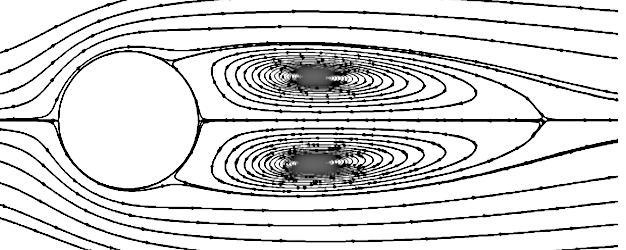
\includegraphics[width=0.43\linewidth,trim=0cm 0cm 0cm 0cm,clip]{flujo_cilindro_visc}};	

	% flux d'air
	\foreach \X in {0,1,...,5}
	{\draw[-latex,line width=.2mm](0,0.5*\X)--++(2*\r,0);};
%	% cylindre
	%\draw[fill=white,ultra thick] (0,0) circle (1);
	\fill[color=white] (2,1.25) circle [radius= \r];
	\draw[fill,pattern=north east lines] (2,1.25) circle [radius= \r];
%	vortex
\draw(6,2.87)-++(.0001,0);
%    \draw [domain=1.15:10,variable=\t,smooth,samples=500,shift={(C)},rotate=20,scale=.9,xshift=1cm,yshift=-0.25cm]
%plot ({-\t r}: {-.02-.83*exp(-.4*\t});
%    \draw [domain=1.25:10,variable=\t,smooth,samples=500,shift={(C)},rotate=-20,scale=.9,xshift=1.75cm,yshift=0.5cm]
%plot ({\t r}: {-.02-.83*exp(-.4*\t});
%    \draw [domain=1.3:10,variable=\t,smooth,samples=500,shift={(C)},rotate=20,scale=.9,xshift=2.5cm,yshift=-0.75cm]
%plot ({-\t r}: {-.02-.83*exp(-.4*\t});	

	%\fill[color=white] (0,2) rectangle ++ (1,2);
	%\draw[fill,pattern=north east lines] (0,-1) rectangle ++ (1,2);	
\end{tikzpicture}
%	\draw[->] (-3.9,-1.5) -- (-3.1,-1.5);
%	\draw[->] (-3.9,-0.5) -- (-3.1,-0.5);
%	\draw[->] (-3.9,0.5) -- (-3.1,0.5);
%	\draw[->] (-3.9,1.5) -- (-3.1,1.5);
%	\node () at (-3.5,2) {$u_\infty$};
%				
%	% LR
%%	\draw[fill=gray!20] (1,0) ellipse (1.9 and 0.9);
%%	\draw[<->] (0,1.5) -- (2.,1.5);
%	\draw[<->] (1,1.5) .. controls (1.1,1.495) and (2.5,1.4)  .. (3.,1.3);
%	\node () at (2.,1.8) {$\ell$};
%	\draw[dashed] (3.,0.8) -- (3.,1.3);
%	\draw[dashed] (1,0) -- (1,1.5);
%	
%	% cylindre
%	%\draw[fill=white,ultra thick] (0,0) circle (1);
%	\draw[fill,pattern=north east lines] (0,0) circle [radius= 1];
%	\fill[color=white] (0,-1) rectangle ++ (1,2);
%	\draw[fill,pattern=north east lines] (0,-1) rectangle ++ (1,2);	
%	
%	
%	\draw[<->] (-1,-1.5) -- (1,-1.5);
%	\node () at (0,-1.8) {$d$};
%	\draw[dashed] (-1,0) -- (-1,-1.5);
%	\draw[dashed] (1,0) -- (1,-1.5);				
%	% 'actuacion' (plasma)
%	\draw[-, thick] (1,1) .. controls (2.5,.9)  .. (3.,.8);
%%	\node () at (0.5,1.3) {$\delta u$};
%%	\draw[-] (0,-1) -- (2.,-1);
%	\draw[-,thick] (1,-1) .. controls (2.5,-.9)  .. (3.,-.8);
%	
%    \draw [domain=1:10,variable=\t,smooth,samples=500,shift={(3.5 ,-.22)},rotate=20,scale=.9]
%plot ({\t r}: {-.02-.83*exp(-.4*\t});
%
%    \draw [domain=1:10, variable=\t,smooth,samples=500,shift={(4.5 ,.22)},rotate=-20,yscale=-1,scale=.9]
%plot ({\t r}: {-.02-.83*exp(-.4*\t});
%
%
%	% axes
%	\draw[black!30][->] (-2.5,0) -- (4.2,0);
%	\node () at (4.3,0) {$x$};
%	\draw[black!30][->] (0,-2) -- (0,2);
%	\node () at (0,2.3) {$y$};
	
%\end{tikzpicture}
%\end{document}	}}
		\subcaption{}\label{fig:cyl}
	\end{subfigure}\hfill
	\begin{subfigure}{.49\textwidth}
	\fbox{\resizebox{\columnwidth}{!}{%
			
\begin{tikzpicture}
	\tikzmath{\r=0.0017*\linewidth;} 
\coordinate (C) at (2,1.25);

% taneda
\node[xshift=0.3\linewidth,yshift=0.034\linewidth] (wake1) at (C.east) {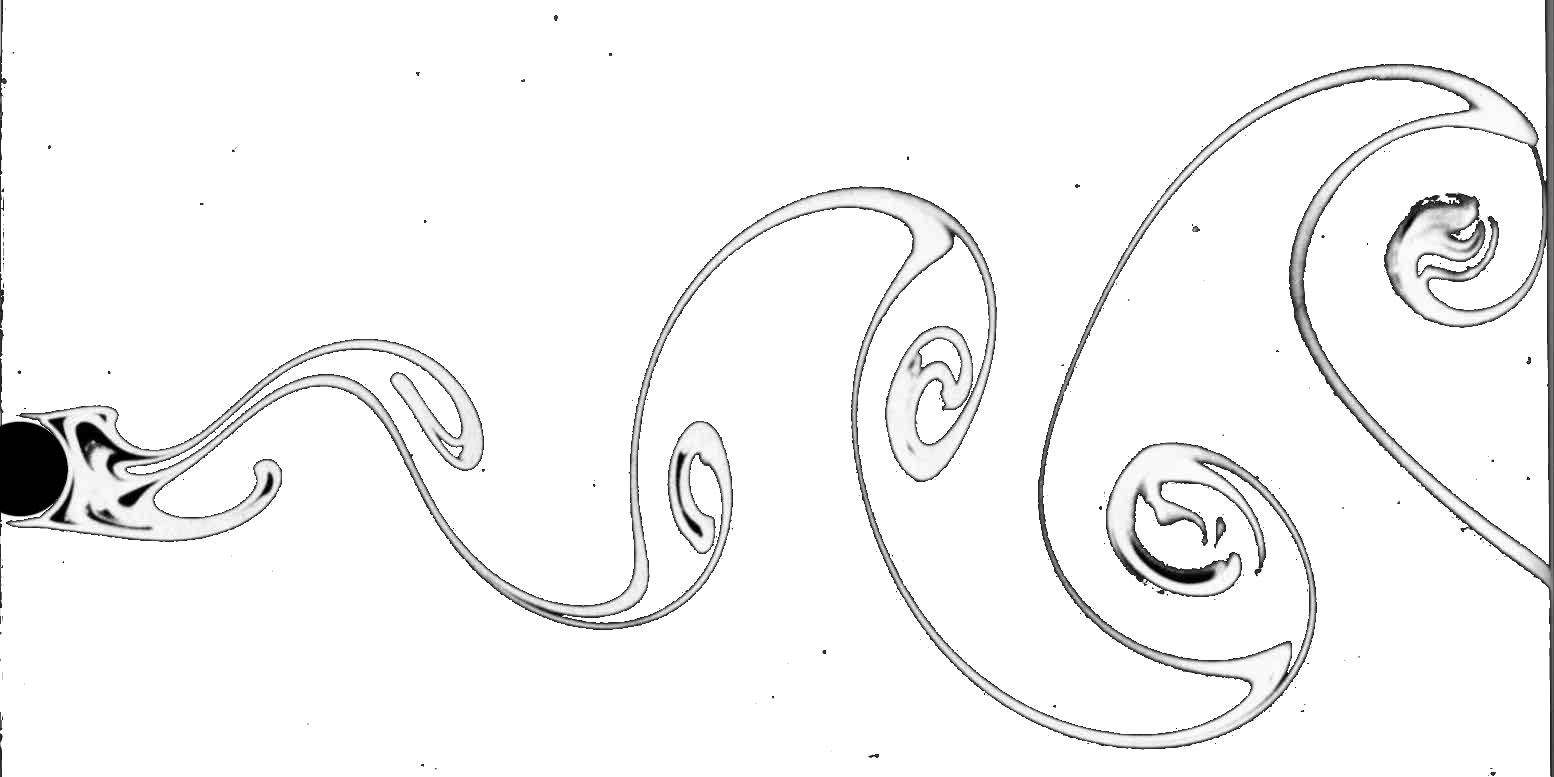
\includegraphics[width=0.51\linewidth,trim=1cm 1cm 7cm 2cm,clip]{benard_taneda_1}};	

	% flux d'air
	\foreach \X in {0,1,...,5}
	{\draw[-latex,line width=.2mm](0,0.5*\X)--++(2*\r,0);};
%	% cylindre
	%\draw[fill=white,ultra thick] (0,0) circle (1);
	\fill[color=white] (2,1.25) circle [radius= \r];
	\draw[fill,pattern=north east lines] (2,1.25) circle [radius= \r];
%	vortex
%    \draw [domain=1.15:10,variable=\t,smooth,samples=500,shift={(C)},rotate=20,scale=.9,xshift=1cm,yshift=-0.25cm]
%plot ({-\t r}: {-.02-.83*exp(-.4*\t});
%    \draw [domain=1.25:10,variable=\t,smooth,samples=500,shift={(C)},rotate=-20,scale=.9,xshift=1.75cm,yshift=0.5cm]
%plot ({\t r}: {-.02-.83*exp(-.4*\t});
%    \draw [domain=1.3:10,variable=\t,smooth,samples=500,shift={(C)},rotate=20,scale=.9,xshift=2.5cm,yshift=-0.75cm]
%plot ({-\t r}: {-.02-.83*exp(-.4*\t});	

	%\fill[color=white] (0,2) rectangle ++ (1,2);
	%\draw[fill,pattern=north east lines] (0,-1) rectangle ++ (1,2);	
\end{tikzpicture}
%	\draw[->] (-3.9,-1.5) -- (-3.1,-1.5);
%	\draw[->] (-3.9,-0.5) -- (-3.1,-0.5);
%	\draw[->] (-3.9,0.5) -- (-3.1,0.5);
%	\draw[->] (-3.9,1.5) -- (-3.1,1.5);
%	\node () at (-3.5,2) {$u_\infty$};
%				
%	% LR
%%	\draw[fill=gray!20] (1,0) ellipse (1.9 and 0.9);
%%	\draw[<->] (0,1.5) -- (2.,1.5);
%	\draw[<->] (1,1.5) .. controls (1.1,1.495) and (2.5,1.4)  .. (3.,1.3);
%	\node () at (2.,1.8) {$\ell$};
%	\draw[dashed] (3.,0.8) -- (3.,1.3);
%	\draw[dashed] (1,0) -- (1,1.5);
%	
%	% cylindre
%	%\draw[fill=white,ultra thick] (0,0) circle (1);
%	\draw[fill,pattern=north east lines] (0,0) circle [radius= 1];
%	\fill[color=white] (0,-1) rectangle ++ (1,2);
%	\draw[fill,pattern=north east lines] (0,-1) rectangle ++ (1,2);	
%	
%	
%	\draw[<->] (-1,-1.5) -- (1,-1.5);
%	\node () at (0,-1.8) {$d$};
%	\draw[dashed] (-1,0) -- (-1,-1.5);
%	\draw[dashed] (1,0) -- (1,-1.5);				
%	% 'actuacion' (plasma)
%	\draw[-, thick] (1,1) .. controls (2.5,.9)  .. (3.,.8);
%%	\node () at (0.5,1.3) {$\delta u$};
%%	\draw[-] (0,-1) -- (2.,-1);
%	\draw[-,thick] (1,-1) .. controls (2.5,-.9)  .. (3.,-.8);
%	
%    \draw [domain=1:10,variable=\t,smooth,samples=500,shift={(3.5 ,-.22)},rotate=20,scale=.9]
%plot ({\t r}: {-.02-.83*exp(-.4*\t});
%
%    \draw [domain=1:10, variable=\t,smooth,samples=500,shift={(4.5 ,.22)},rotate=-20,yscale=-1,scale=.9]
%plot ({\t r}: {-.02-.83*exp(-.4*\t});
%
%
%	% axes
%	\draw[black!30][->] (-2.5,0) -- (4.2,0);
%	\node () at (4.3,0) {$x$};
%	\draw[black!30][->] (0,-2) -- (0,2);
%	\node () at (0,2.3) {$y$};
	
%\end{tikzpicture}
%\end{document}	}}
	\subcaption{}\label{fig:bvk}
	\end{subfigure}\hfill

	\caption{(a) Lineas de corriente del desprendimiento de la capa límite en flujo viscoso. (b) Visualización de la calle de vórtices de Bénard-von Kármán.}\label{fig:cylinder_flow}

\end{figure}



 Por un lado, desde el análisis de los cambios en la estructura coherente\footnote{ De su definición (ver, por ejemplo \cite{hussain1986}), las estructuras coherentes son regiones de un escurrimiento que conservan su forma y comportamiento aún si se establecen regímenes turbulentos.} con la que se conoce a la inestabilidad de la estela: la calle de vórtices de Bénard-Von Kármán.  Se la modela como un modo global \cite{zielinska,barkley2006} que define espacial y temporalmente al escurrimiento. Se puede conseguir una descripción como modelo reducido alrededor del valor crítico $\mathrm{Re_c}$ a partir del planteo de la evolución desde la ecuación de Stuart-Landau\cite{stuart58, provansal1987} que puede derivarse de métodos más generales \cite{noack2003a,dadamo2007}.
 
 
 Lejos del umbral, \citet{gallaire2016} demostraron  la pertinencia del modo global, confirmando estudios previos\cite{barkley2006,sipp2007}. En nuestro trabajo \cite{boury2018forced} extendimos el análisis a casos forzados por actuación externa, completando formalmente una propuesta de \cite{thiria2007}. Habíamos también  estudiado la acción de control mediante actuadores plasma\cite{dadamo2012} a $\mathrm{Re}\sim 200$ y en \cite{boury2018forced} conseguimos formular un modelo a través de la ecuación de Landau que las incluye. También, en \citet{dadamo2017a}, basándonos en conceptos de modelos reducidos y modos globales, aplicamos control a mayores números de Reynolds ($\sim 5000$).
 
  Es de notar que pueden modelarse las acciones de control a través de las modificaciones del campo medio del flujo, independientemente de cual sea su origen. Mediante control mecánico, de oscilaciones rotatorias  como el que estudiamos en \cite{dadamo2011b} se pueden conseguir resultados semejantes.

 Para flujos de estela cuando $\mathrm{Re}>180$, el flujo deja de ser bidimensional abriendo posibilidades de sucesivas bifurcaciones y transiciones típicas de turbulencia. También pueden desencadenarse estos procesos a través del control, como observaban \cite{thiria2007,dadamo2011b} y confirmamos en \cite{dadamo2015a}, distinguiendo el modo fundamental de bifurcación asociado a una inestabilidad centrífuga. 
 
 Otro concepto relevante a la hora de caracterizar flujos de estela es el de \textit{resonancia}. Aparece vinculado primeramente a la frecuencia dominante de una estela, la que corresponde al desprendimiento de vórtices $f_{vs}$ dada por el número de Strouhal $\mathrm{St}=f_{vs}D/U$. Pero aún sin desprendimiento de vórtices, existe una frecuencia que es la que corresponde a las oscilaciones globales que surgen como consecuencia de perturbaciones al flujo base, que es el campo estacionario de velocidades. 
 
 La teoría de inestabilidad hidrodinámica cuenta con numerosos antecedentes experimentales, teóricos desde el siglo XIX y principios del siglo XX, con los aportes de Kelvin, Rayleigh, Reynolds, Bénard, von Kármán y Taylor entre otros. En particular, los trabajos de Landau\cite{landau1985} sobre ondas en plasmas en la década de 1940 formalizaron la teoría que más tarde fue aplicada a mecánica de fluidos en distintos problemas canónicos\cite{gaster1965role,mattingly1972stability,huerre1985absolute,trianta1986}. Se desarrolla así el concepto de frecuencia de resonancia de un campo de velocidades, como aquella propia de una perturbación que sufre la mayor amplificación temporal o espacial. Así como existen frecuencias de perturbaciones o números de ondas asociados, éstos definen también regiones espaciales que son más receptivas a ser perturbadas. Al respecto, el trabajo experimental de \cite{strykowski1990formation} describe 
 
Recientemente,  \citet{herrmann2020modeling} extienden y evalúan la capacidad de modelos reducidos de responder en estas situaciones con resultados alentadores para el diseño de estrategias de control eficaces.
 

 \subsection*{Interacción fluido-estructura}
 
 Además de las estrategias de control \textit{activo }\footnote{Se distingue al control activo por ser métodos en los que se introduce energía externa a un sistema mientras que en control pasivo, la acción de control se diseña como una respuesta propia del sistema. } mencionadas, nos interesamos particularmente en problemas donde existe un fuerte acople entre la mecánica de fluidos y la de sólidos con deformaciones  elásticas.	
 	
Suceden distintos grados de interacción de acuerdo a los tiempos característicos propios de cada medio. Pueden clasificarse (ver por ejemplo \cite{paidoussis2010fluid,delangre2001fluides}) comparando números adimensionales de cada caso y eventualmente aquellos característicos del acople.
Entre estos últimos,  los principales que suelen plantearse son: la velocidad reducida $U_R=U_{sol}/U_{fl}$; el número de masa $\mathcal{M}=\rho_f/\rho_s$ y el número de Cauchy $C_Y=\rho_fU_{fl}^2/E$ que se suman a los números propios de la mecánica de fluidos (típicamente, el Número de Reynolds, $\mathrm{Re}=UL/\nu$, el número de Strouhal $\mathrm{St}=fU/L$, etc.) y del sólido (desplazamientos relativos $\delta/L$, deformaciones elásticas $\varepsilon=\sigma/E$, etc.). 

Un caso particular de escurrimiento de estela con fuerte interacción fluido estructura es el que producen alas batientes.  Estudios sobre animales voladores o nadadores de alas batientes\cite{Dickson:2004p232,harrison2000} han demostrado que éstos utilizan las propiedades flexibles de sus miembros para optimizar sus desplazamientos. A través de biomimetismo, se pueden volcar conceptos para el diseño en ingeniería. En este sentido,
diversos trabajos\cite{marais2012,ramananarivo2011a,dewey2013,paraz2016thrust} exploraron el rol de la flexibilidad y como se modifica el problema de resonancia mecánica
considerando el sistema placas flexibles y fluido. Pueden distinguirse dos tipos principales de movimiento, el de cabeceo, oscilaciones angulares, y agitado, oscilaciones en la dirección  normal al flujo (\textit{pitching} y \textit{heaving} en inglés, respectivamente).

En alas batientes , el tamaño característico resulta de considerar nuevamente la dimensión normal al flujo. Si se consideran oscilaciones angulares ($\theta$) rotatorias del tipo $\theta = \theta_0\sin(\omega t)$, de frecuencia $f_f = \omega/2\pi$, y un largo o cuerda de ala $\mathscr C$, dicho tamaño es $A=\mathscr{C} \sin(\theta_0)$. Así, el número de Strouhal asociado es $\mathrm{St}=f_f A / U$ y pensando en un coeficiente de propulsión\footnote{Es el opuesto al coeficiente de arrastre.} $C_T=2\mathscr{F}_T/(\rho U^2 A L_z)$, para alas de envergadura $L_z$. Aparece asociado a estos números el problema de conseguir propulsiones eficientes pensando en aplicaciones de locomoción o bien, invirtiéndolo, en mecanismos capaces de generar energía a partir de un escurrimiento.

Los criterios para lograr soluciones óptimas de propulsión de alas flexibles han sido objeto de debate en los últimos 15 años.  Particularmente, a partir de una propuesta de \citet{Triantafyllou:2002p282},  \citet{moored2012hydrodynamic} relacionaron el rol de la estabilidad hidrodinámica de la estela con el forzado y la dinámica de las placas batientes  que la producen. Resolviendo la ecuación de Orr-Somerfeld en forma \textit{local}, los autores extraen un conjunto de frecuencias  y modos que se encuentran asociados a los casos de mayor eficacia de las fuerzas de propulsión. Tratándose de un experimento en agua, con $\mathcal{M}\sim 1$, a números de Reynolds \textit{moderados}, a la inestabilidad invíscida propia del gradiente de velocidades en la estela, se suman efectos  de difusión viscosa y de masas virtuales. 
En una publicación reciente\cite{dadamo2022wake}, abordamos el estudio de  optimización de la propulsión para placas flexibles en flujos de aire, $\mathcal{M}\ll 1$. Entre otros resultados, se observa claramente la relación entre el fenómeno de resonancia de la estela\cite{chomaz2005}, de inestabilidad invíscida\cite{charru2012instabilites}, respecto al modo de vibración elástica. Este aspecto ayudará en la elaboración de estrategias de control en la geometría y en otras más complejas como puede ser  la estela de un cuerpo romo asociada a la dinámica de una placa flexible  propulsora.

En efecto, un aspecto que estudiaremos en profundidad será el de la reducción o el aumento de arrastre en cuerpos romos a partir del movimiento o de la reconfiguración de placas flexibles\cite{gosselin2010drag}. Estudios previos numéricos\cite{wu2016characteristics} mostraron que se pueden conseguir reducciones del orden del 50\% para la estela de un cilindro. Más recientemente, \citet{garcia2021drag} mostraron resultados experimentales para más altos números de Reynolds, en vistas de la aplicación en transporte terrestre. Si bien realizan un análisis para vincular la elasticidad de la placa con reducciones de arrastre (14\%) y de fluctuaciones, quedan aspectos clave por responder y que podrían mejorar los resultados obtenidos.

\bibliographystyle{unsrtnat}
\begin{small}
\bibliography{/home/juan/Documents/bibtex/citas.bib}	
\end{small}

\end{document}
